\documentclass{beamer}
\usepackage{bm}
\usepackage{adjustbox}
\usepackage{multimedia}
\usepackage{animate}
\usepackage{tikz}
\usetikzlibrary{snakes}

\setbeamerfont{caption}{size=\footnotesize}

%Information to be included in the title page:
\title{Control of Go1}
\subtitle{And overview of first 2 weeks}
\author{Andrew Stirling}
\institute{Berliner Hoschule fur Teknik}
\date{}

\begin{document}

\frame{\titlepage}

\begin{frame}
    \frametitle{Timeline}
    \begin{center}
        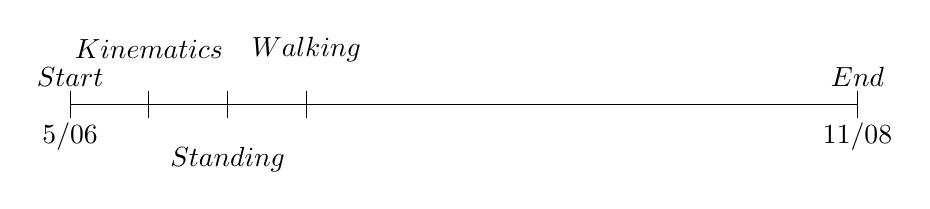
\begin{tikzpicture}[snake=zigzag]
        % draw horizontal line   
        \draw (0,0) -- (10,0);
 

        % draw vertical lines
        \foreach \x in {0,1,2,3,10}
            \draw (\x cm,5pt) -- (\x cm,-5pt);

        % draw nodes
        \draw (0,0) node[below=3pt] {$ 5/06 $} node[above=3pt] {$ Start $};
        \draw (1,0) node[below=3pt] {$  $} node[above=13pt] {$ Kinematics $};
        \draw (2,0) node[below=3pt] {$  $} node[below=12pt] {$ Standing $};
        \draw (3,0) node[below=3pt] {$  $} node[above=12pt] {$ Walking $};
        \draw (10,0) node[below=3pt] {$ 11/08 $} node[above=3pt] {$ End $};
        \end{tikzpicture}
    \end{center}
        
\end{frame}

\begin{frame}
    \begin{columns}[T]
        \begin{column}{.55\textwidth}
         \begin{block}{Forward Kinematics}
            \begin{align*}
                &x = L_t sin(\theta_t) + L_c sin(\theta_t + \theta_c) \\
                &z = [L_t cos(\theta_t) + L_c cos(\theta_t + \theta_c)]cos(\theta_h) \\
                &y = ztan(\theta_h)\\
            \end{align*}
            Where
            $L_c = $ Length of Calf \\
            $L_t =$ Length of Thigh \\
            $\theta_c=$ Calf Angle 
            $\theta_t=$ Thigh Angle \\
            $\theta_h =$ Hip Angle 
        \end{block}
        \end{column}
        \begin{column}{.45\textwidth}
        \begin{block}{}
    % Your image included here
        \begin{figure}
            \includegraphics[width=0.9\textwidth, height=0.5\textheight]{../images/coords_fix.png}
            \caption{Go1 Coordinate Axes}
        \end{figure}
        \end{block}
        \end{column}
      \end{columns}

\end{frame}

\begin{frame}
    \begin{columns}[T]
        \begin{column}{.55\textwidth}
         \begin{block}{Inverse Kinematics}

            $L_c = $ Length of Calf \\
            $L_t =$ Length of Thigh \\
            $\theta_c=$ Calf Angle \\
            $\theta_t=$ Thigh Angle \\
            $\theta_h =$ Hip Angle \\
            ;\ \\
            \begin{align*}
                &\theta_h = arctan(\frac{y}{z})\\
                &\theta_c = arcsin(\frac{x}{L} - sin(\theta_t)) - \theta_t \\
                &\theta_t = arccos(\frac{\sqrt{x^2 + y^2 + z^2}}{L_t + L_c}) + arctan(\frac{-x}{\sqrt{y^2 + z^2}}) \\
            \end{align*}

        \end{block}
        \end{column}
        \begin{column}{.45\textwidth}
        \begin{block}{}
    % Your image included here
        \begin{figure}
            \includegraphics[width=0.9\textwidth, height=0.5\textheight]{../images/coords_fix.png}
            \caption{Go1 Coordinate Axes}
        \end{figure}
        \end{block}
        \end{column}
      \end{columns}

\end{frame}

\begin{frame}
    \frametitle{Standing Controller}
    \begin{columns}[onlytextwidth, T]
        \begin{column}{.4\textwidth}
            Gravity Compensated PD-Controller
            \begin{align*}
                \bm{\tau} = \bm{J^T}&(\bm{\theta})\cdot \bm{F_{gc}} \\
                & + K_p \bm{\theta_e} + K_d \bm{\dot{\theta_d}} \\ 
            \end{align*}
            Position of feet statically set to 
            $ \vec{p} = \begin{bmatrix}
                -0.02 \\
                0.02 \\
                -0.3
              \end{bmatrix}$ \\
              With respect to coordinate system above. Gains were also set
              for each joint as $ K_p = 30; K_d = 0.1$
        \end{column}
        \begin{column}{.7\textwidth}
            \begin{figure}
                \includegraphics[height=0.4\textheight]{../images/torques.png}
                % \caption{Joint Torques}
            \end{figure}
            \vspace{-0.9cm}
            \begin{figure}
                \includegraphics[height=0.4\textheight]{../images/com.png}
                % \caption{Center of Mass Position}
            \end{figure}
        
        \end{column}
      \end{columns}
\end{frame}

\begin{frame}
    \frametitle{Walking Controller}
    \begin{columns}[onlytextwidth, T]
        \begin{column}{.4\textwidth}
            Feet trajectory generated using Bezier Curves. \\

            $\bm{F_{gc}}$ now contains weight of body split between the two "standing" legs.
            And weight of the leg itself for "swinging" legs. \\
            
            Gains set to $K_p = 50$ and $K_d = 1 $ in walking state.
        \end{column}
        \begin{column}{.6\textwidth}
            \begin{figure}
                \includegraphics[height=0.6\textheight]{../images/traj.png}
                % \caption{Joint Torques}
            \end{figure}

        
        \end{column}
      \end{columns}
\end{frame}

\begin{frame}
    \frametitle{Standing Controller}
    \begin{columns}[onlytextwidth, T]
        \begin{column}{.5\textwidth}
            \begin{figure}
                \includegraphics[height=0.3\textheight]{../images/w_torque.png}
            \end{figure}
            \vspace{-0.9cm}
            \begin{figure}
                \includegraphics[height=0.4\textheight, width=\textwidth]{../images/zoom_torque.png}
                \caption{Joint Torques}
            \end{figure}
            
        \end{column}
        \begin{column}{.5\textwidth}
            \begin{figure}
                \includegraphics[width=\textwidth]{../images/rms.png}
                \caption[font=tiny]{Root Mean Square of Torques}
            \end{figure}
            \vspace{-0.9cm}
            \begin{figure}
                \includegraphics[height=0.4\textheight]{../images/w_com.png}
                \caption{Center of Mass Position}
            \end{figure}
        \end{column}
      \end{columns}
\end{frame}
\begin{frame}
    \frametitle{Next Steps}
    \begin{itemize}
      \item Implement standing procedure.
      \item Implement variable step-length of each leg so can have a controller to adjust
      position if path isn't straight.
      \item Tune gains of each individual joint and general controller improvement. 
      \item Apply neural net to "learn" control. 
    \end{itemize}
  \end{frame}

\begin{frame}
    \frametitle{Roadblocks}
    \begin{itemize}
      \item Physical low-level control of Go1, hopefully fixed with new board.
    \end{itemize}
  \end{frame}

\end{document}

